% =====================================================================
%  BreathNote: Smart Incentive Spirometer
%  Concept document for the National Student Ideation Challenge
%
%  Compile with pdfLaTeX (run twice so page numbers settle):
%      pdflatex proposal.tex
%      pdflatex proposal.tex
% =====================================================================
\documentclass[12pt,a4paper]{article}

% ---------- Page layout ----------------------------------------------
\usepackage[a4paper, margin=2.5cm]{geometry}

% ---------- Fonts ----------------------------------------------------
\usepackage[T1]{fontenc}
\usepackage{textcomp}
\usepackage{tgtermes}                   % Times-style serif for all text
\usepackage{microtype}
\linespread{1.03}

\newcommand{\rupee}{Rs.\,}              % currency prefix used in the text

% ---------- Paragraphs, lists, headings ------------------------------
\setlength{\parindent}{0pt}
\setlength{\parskip}{6pt}
\widowpenalty=10000
\clubpenalty=10000

\usepackage{enumitem}
\setlist{itemsep=2pt, topsep=4pt, parsep=0pt, leftmargin=1.5em}

\usepackage{titlesec}
\titleformat{\section}{\normalfont\large\bfseries}{\thesection.}{0.5em}{}
\titlespacing*{\section}{0pt}{16pt}{6pt}
\titleformat{\subsection}{\normalfont\normalsize\bfseries}{\thesubsection}{0.5em}{}
\titlespacing*{\subsection}{0pt}{10pt}{4pt}

% ---------- Tables and figures ---------------------------------------
\usepackage{array, booktabs, tabularx}
\renewcommand{\arraystretch}{1.2}
\newcolumntype{L}{>{\raggedright\arraybackslash\hyphenpenalty=10000}X}
\newcolumntype{P}[1]{>{\raggedright\arraybackslash\hyphenpenalty=10000}p{#1}}

\usepackage{graphicx}
\usepackage{float}                      % [H] keeps a table under its heading
\usepackage{needspace}                  % keeps a heading with its table
\usepackage{caption}
\captionsetup{font=small, labelfont=bf, labelsep=colon, skip=6pt}
\captionsetup[table]{position=top}

\usepackage{tikz}
\usetikzlibrary{positioning, arrows.meta, calc}

% ---------- Page numbers ---------------------------------------------
\usepackage{fancyhdr, lastpage}
\pagestyle{fancy}
\fancyhf{}
\fancyfoot[C]{\small Page \thepage{} of \pageref{LastPage}}
\renewcommand{\headrulewidth}{0pt}
\fancypagestyle{plain}{\fancyhf{}\fancyfoot[C]{\small Page \thepage{} of \pageref{LastPage}}}

% ---------- Links (printed in black) ---------------------------------
\usepackage[hidelinks]{hyperref}
\hypersetup{
  pdftitle={BreathNote: A Smart Incentive Spirometer with Breath-Driven Music Feedback},
  pdfauthor={Ande Karthik, Kalluri Roshan Lal, Pasumarthy Deepak}}
\urlstyle{same}

% ---------- Project details (edit here) ------------------------------
\newcommand{\githuburl}{https://github.com/Roshan-o/Spirometer}
\newcommand{\videourl}{https://drive.google.com/file/d/18UdDUZlwO37Ve3utC2zd_bIKU9YbzDy5/view}

% =====================================================================
\begin{document}
\thispagestyle{plain}

% ---------- Title block ----------------------------------------------
\begin{center}
  {\LARGE\bfseries BreathNote\par}
  \vspace{6pt}
  {\Large A Smart Incentive Spirometer with\\ Breath-Driven Music Feedback\par}
  \vspace{14pt}
  {\normalsize
  \begin{tabular}{@{}c@{\hspace{2.2em}}c@{\hspace{2.2em}}c@{}}
    Ande Karthik & Kalluri Roshan Lal & Pasumarthy Deepak \\
    2023102009   & 2023102010         & 2023101109
  \end{tabular}\\[8pt]
  International Institute of Information Technology, Hyderabad\\[2pt]
  November 2026\par}
\end{center}
\vspace{6pt}

% =====================================================================
\section*{Overview}

Patients recovering from surgery or lung illness are asked to use an incentive spirometer about ten times every waking hour. The exercise is repetitive and boring, so many patients skip it. The device also records nothing, so the doctor cannot see how the patient is doing from day to day.

BreathNote is a low-cost sensor add-on for the standard 3-ball incentive spirometer, connected to a web application. The patient's breath controls the music feedback, a continuous frequency glide that builds into a 3-part harmony, which makes the exercise engaging. Every session is recorded, and the patient's daily metrics are tracked on a personal dashboard. The patient can download a progress report and receives reminder notifications for each exercise. As a planned enhancement, reports will be sent directly to the doctor for remote monitoring.

A working prototype has been built and tested end to end. It costs about \rupee 1,150--1,750 per unit. We seek a hospital partner for a pilot study, clinical mentorship and funding for high-accuracy airflow sensors.

% =====================================================================
\section{Problem Statement}

After surgery, or while recovering from a lung illness, patients are asked to use an \textbf{incentive spirometer}. It is a simple plastic device with three balls. The patient breathes in slowly and deeply, and the balls rise. Regular deep breathing helps the lungs expand fully and lowers the risk of collapsed air sacs (atelectasis) and pneumonia.

The exercise must be repeated very often. A common hospital instruction is about \textbf{10 deep breaths every hour while awake} \cite{cleveland}. That is more than 100 breaths a day, for the whole recovery period. This leads to four problems:

\begin{enumerate}
  \item \textbf{The exercise is boring.} The same action is repeated with no change, so patients lose interest. Many do it wrongly or stop using the device.
  \item \textbf{The device gives no motivation.} It only shows balls moving up. There is no sound, no reward and no reason to keep going.
  \item \textbf{Nothing is recorded.} The device does not save how hard the patient breathed, how long they held the breath or how often they practised. Patients cannot see their own improvement.
  \item \textbf{The doctor cannot follow daily progress.} Between visits, the doctor has no information on how the patient is doing each day. There are no metrics, no tracking and no report. A patient who skips the exercise or stops improving is noticed late.
\end{enumerate}

\textbf{Who is affected.} Patients after chest, heart or abdominal surgery; patients with COPD, asthma or other conditions that cause shallow breathing; and elderly patients or people on long bed rest. Doctors, nurses and physiotherapists are also affected, because they cannot see whether patients practise. The problem occurs in surgical wards, ICUs and rehabilitation centres, and most of all at home after discharge, where nobody supervises the exercise.

\textbf{Scale of the problem.} Lung disease affects low- and middle-income countries, including India, the most. The following figures are reported in \cite{wallace}, based on World Health Organization and Global Burden of Disease data:

\begin{itemize}
  \item \textbf{More than 90\%} of deaths from chronic obstructive pulmonary disease (COPD) among people under 70 occur in low- and middle-income countries.
  \item \textbf{96\%} of global asthma deaths in 2019 occurred in these countries.
\end{itemize}

A low-cost, engaging and trackable device therefore matters most in such settings, including India's district hospitals, rural health centres and homes.

The medical exercise itself works. The problem is that the device does not keep patients engaged, does not measure what they do, and does not tell the doctor how they are progressing.

% =====================================================================
\section{Proposed Solution}

BreathNote is a \textbf{Smart Incentive Spirometer}. We fit a small, low-cost pressure sensor into a normal 3-ball incentive spirometer and connect it to a web application. The application turns each breath into music feedback, shows live visual feedback, and records every session. It has four parts:

\begin{itemize}
  \item \textbf{Sensor add-on:} fits the spirometer that hospitals and patients already use, so nobody has to learn a new device.
  \item \textbf{Web application:} secure login, a live breathing screen and a personal dashboard.
  \item \textbf{Music feedback:} a breath-driven glide of musical notes that builds into a 3-part harmony.
  \item \textbf{Daily tracking and reports:} the patient's daily metrics are recorded, a progress report can be downloaded, and reminder notifications prompt each exercise.
\end{itemize}

\begin{figure}[h]
  \centering
  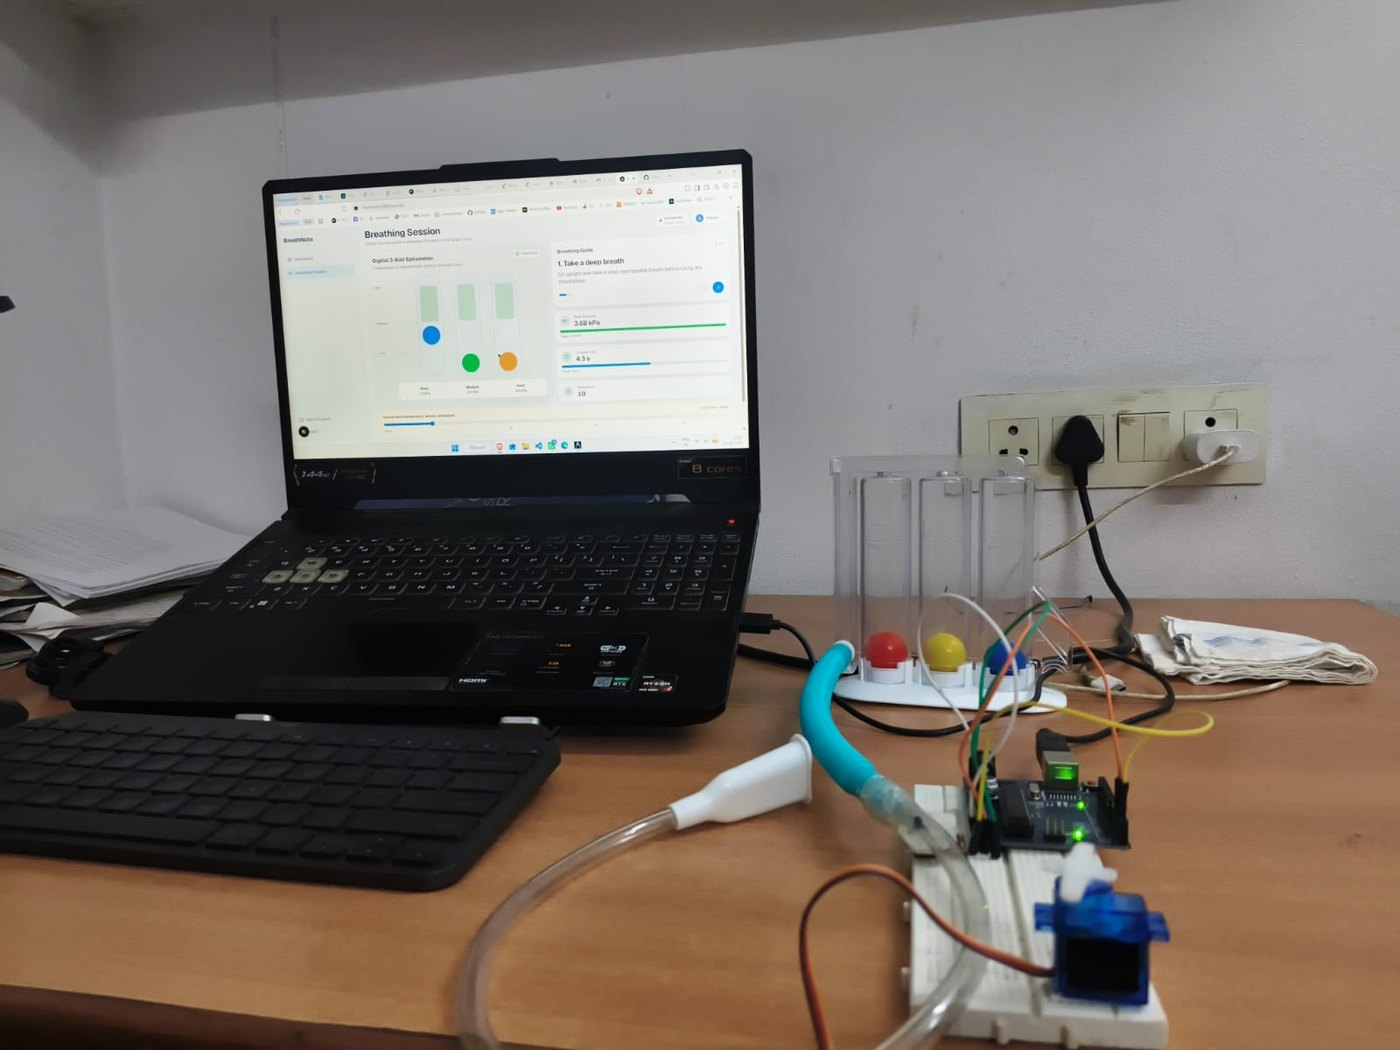
\includegraphics[width=0.62\linewidth]{figures/prototype.jpg}
  \caption{The working prototype: a standard 3-ball incentive spirometer with a pressure sensor in its tube, an Arduino, and the live breathing session on a laptop.}
  \label{fig:prototype}
\end{figure}

\textbf{Why music.} Music is already used as a live reward in medical devices, for example MedRhythms for walking rehabilitation \cite{medrhythms} and the Pacifier Activated Lullaby for newborn feeding \cite{pal}. A study on music biofeedback found that music changed breathing only when it responded to the user's breath; music played in the background had no effect \cite{bhandari}. In BreathNote, therefore, the breath itself controls the music. Music with smooth gliding notes holds attention and suits slow, deep breathing.

\textbf{Daily tracking and reports.} Every session is saved with its metrics: number of repetitions, peak pressure, highest level reached, longest hold and session time. The dashboard shows these day by day, with a progress chart and a 14-day consistency tracker. This gives a clear record of how the patient is doing each day. The patient can \textbf{download a progress report} at any time and share it with the doctor, and \textbf{reminder notifications} prompt the patient to do each exercise on time. As a planned enhancement, the report will be \textbf{sent directly to the doctor}, so the doctor can monitor recovery remotely without an extra visit.

% =====================================================================
\section{Working of the System}

\begin{figure}[h]
\centering
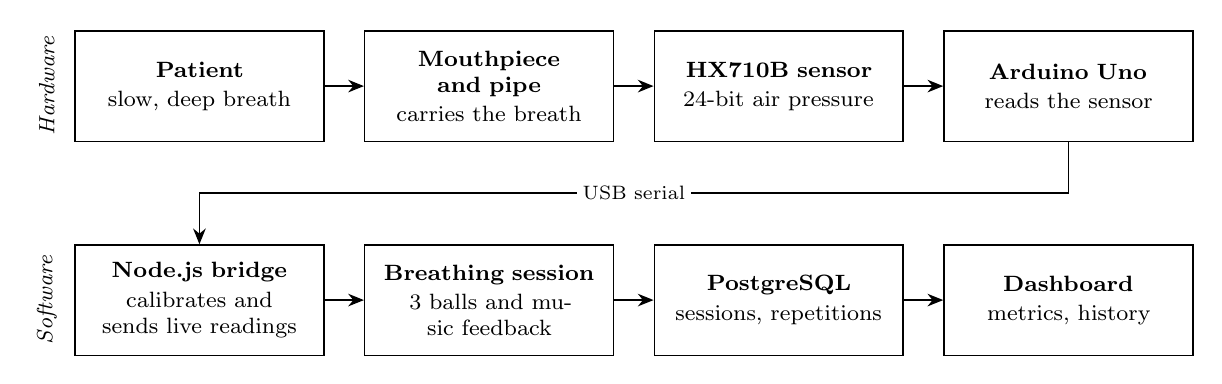
\begin{tikzpicture}[
    node distance=5mm,
    box/.style={draw=black, fill=white, line width=0.5pt, align=center,
                text width=2.95cm, minimum height=14mm, inner sep=3pt,
                font=\footnotesize},
    arr/.style={-{Stealth[length=2mm, width=1.6mm]}, line width=0.6pt},
    lane/.style={rotate=90, font=\footnotesize\itshape}
  ]
  % Hardware row
  \node[box]                (a1) {\textbf{Patient}\\[1pt] slow, deep breath};
  \node[box, right=of a1]   (a2) {\textbf{Mouthpiece and pipe}\\[1pt] carries the breath};
  \node[box, right=of a2]   (a3) {\textbf{HX710B sensor}\\[1pt] 24-bit air pressure};
  \node[box, right=of a3]   (a4) {\textbf{Arduino Uno}\\[1pt] reads the sensor};
  % Software row
  \node[box, below=13mm of a1] (b1) {\textbf{Node.js bridge}\\[1pt] calibrates and sends live readings};
  \node[box, right=of b1]      (b2) {\textbf{Breathing session}\\[1pt] 3 balls and music feedback};
  \node[box, right=of b2]      (b3) {\textbf{PostgreSQL}\\[1pt] sessions, repetitions};
  \node[box, right=of b3]      (b4) {\textbf{Dashboard}\\[1pt] metrics, history};
  % Flow
  \draw[arr] (a1) -- (a2);
  \draw[arr] (a2) -- (a3);
  \draw[arr] (a3) -- (a4);
  \draw[arr] (a4.south) -- ++(0,-6.5mm)
     -| node[pos=0.25, fill=white, inner sep=2pt, font=\scriptsize] {USB serial}
     (b1.north);
  \draw[arr] (b1) -- (b2);
  \draw[arr] (b2) -- (b3);
  \draw[arr] (b3) -- (b4);
  % Row labels
  \node[lane] at ($(a1.west)+(-3.5mm,0)$) {Hardware};
  \node[lane] at ($(b1.west)+(-3.5mm,0)$) {Software};
\end{tikzpicture}
\caption{Data flow from the patient's breath to the dashboard. The bridge streams pressure readings to the browser over a WebSocket.}
\label{fig:flow}
\end{figure}

\begin{enumerate}
  \item \textbf{Breathe.} The patient breathes slowly and deeply through the mouthpiece of a 3-ball incentive spirometer.
  \item \textbf{Sense.} An HX710B air pressure sensor is sealed into a small hole in the tube. The far end of the tube is closed by the spirometer body, so the pressure changes across the whole tube and one sensor point is enough.
  \item \textbf{Read.} An Arduino reads the sensor and sends the values to a laptop over USB.
  \item \textbf{Convert.} A small Node.js bridge learns the zero level in the first 3 seconds, when nobody is breathing. It converts each reading to kPa and streams it live to the browser.
  \item \textbf{Show and play.} The web application smooths the signal, moves three virtual balls and plays a sound that follows them (Table~\ref{tab:music}). It is silent at rest and has a mute button.
  \item \textbf{Count.} A repetition starts when the pressure rises above 0.5~kPa and ends when it falls back. For each repetition, the application records the peak pressure, the highest level and the longest hold.
  \item \textbf{Save and track.} When the session ends, the server checks the data (for example, pressure must be between 0 and 5~kPa) and saves it. The dashboard shows peak pressure, longest hold, average session time, weekly sessions, a progress chart, a 14-day consistency tracker and the full history.
\end{enumerate}

\begin{table}[h]
\centering
\caption{Mapping of spirometer levels to musical feedback (prototype values).}
\label{tab:music}
\small
\begin{tabularx}{\linewidth}{@{}l l l L@{}}
\toprule
\textbf{Ball} & \textbf{Level} & \textbf{Prototype threshold*} & \textbf{Sound as the ball rises} \\
\midrule
Ball 1 (blue)   & Easy   & 1.5 kPa & Soft, breathy noise slowly turns into the first note of the harmony \\
Ball 2 (green)  & Medium & 2.5 kPa & Pitch glides smoothly up to the second note of the harmony \\
Ball 3 (orange) & Hard   & 3.5 kPa & Pitch glides up to the third note, completing the harmony \\
\bottomrule
\end{tabularx}

\vspace{4pt}
\begin{minipage}{\linewidth}\footnotesize
*These thresholds were set for testing the prototype. They are not clinical values. Final thresholds will be set with doctors during the pilot study and can be adjusted for each patient.
\end{minipage}
\end{table}

The patient's breath controls a continuous frequency glider, which plays a 3-part harmony mapped to the 3 columns of the spirometer upon successfully implementing the breathing intensity. This makes the exercise more aesthetically pleasing and engaging.

\textbf{Technology.} Next.js (React, TypeScript) and Tailwind CSS for the web application; Recharts for charts; PostgreSQL on Neon with Prisma for data storage; a Node.js serial-to-WebSocket bridge; and an Arduino for the hardware.

\textbf{Safety and privacy.} Passwords are stored only as bcrypt hashes. Logins use a 7-day token in an HTTP-only cookie. Each user can see only their own data. A session can start only when the real sensor is connected, so every saved record comes from real breathing.

% =====================================================================
\section{Innovation}

\begin{enumerate}
  \item \textbf{The breath plays the music.} The music is not played in the background. The breath drives a smooth glide of musical notes, and a study found that music changes breathing only when it responds to the user \cite{bhandari}.
  \item \textbf{Harmonious music feedback.} The three notes of the harmony, with smooth glides between them, were chosen to sound harmonious and calming, which makes the therapy pleasant. To our knowledge, breath-driven music feedback of this kind has not been built into an incentive spirometer before.
  \item \textbf{It upgrades a device patients already use.} We add a sensor to a standard 3-ball spirometer instead of building a new, costly machine.
  \item \textbf{It tracks daily progress for the doctor.} Every session and repetition is saved, and the patient can download a progress report for the doctor. Sending reports directly to the doctor for remote monitoring is planned.
  \item \textbf{Very low cost, chosen by testing.} We tested several sensing methods and chose the simplest one that works at the low effort levels patients produce (Section~\ref{sec:sensors}).
  \item \textbf{It rewards good technique.} The music climbs only as the patient breathes harder and holds longer. This encourages the slow, sustained breath that doctors want.
\end{enumerate}

\begin{table}[h]
\centering
\caption{Comparison of a conventional incentive spirometer with BreathNote.}
\label{tab:compare}
\small
\begin{tabularx}{\linewidth}{@{}P{3.1cm} L L@{}}
\toprule
\textbf{Feature} & \textbf{Conventional 3-ball spirometer} & \textbf{BreathNote} \\
\midrule
Feedback          & Balls rise (visual only)     & Balls on screen and breath-driven music feedback \\
Motivation        & Only the sight of the balls rising & Balls rising on screen, plus a music reward that grows with effort and hold time \\
Data recorded     & Nothing                      & Every session and repetition: peak pressure, level, hold time \\
Daily tracking    & Not possible                 & Personal dashboard with daily metrics, consistency and history \\
For the doctor    & Only if they watch in person & Daily records and downloadable reports; direct sharing and remote monitoring (planned) \\
Device            & Standard device              & Same device with a low-cost sensor add-on \\
\bottomrule
\end{tabularx}
\end{table}

% =====================================================================
\section{Current Stage and Evidence}

\textbf{Stage: Working prototype.} The hardware, web application, music feedback and dashboard all work together on live sensor data.

\subsection{Work Completed}

\textbf{Hardware.} A pressure sensor is sealed into the breathing pipe and read by an Arduino. Its readings reach the web application live. All test and simulated data has been removed, so every saved session comes from real breathing.

\textbf{Web application.} The breathing screen shows three virtual balls and three levels. Each user has a secure login and a personal dashboard with daily metrics. Users can download a progress report, and exercise reminder notifications prompt them to practise on time.

\textbf{Music feedback.} The frequency glider plays a 3-part harmony. Each note follows one of the rising balls, and together they sound harmonious.

\textbf{Calibration and testing.} The sensor has been calibrated against a real 3-ball spirometer, and the complete system has been tested end to end (Section~\ref{sec:testing}).

\begin{figure}[H]
  \centering
  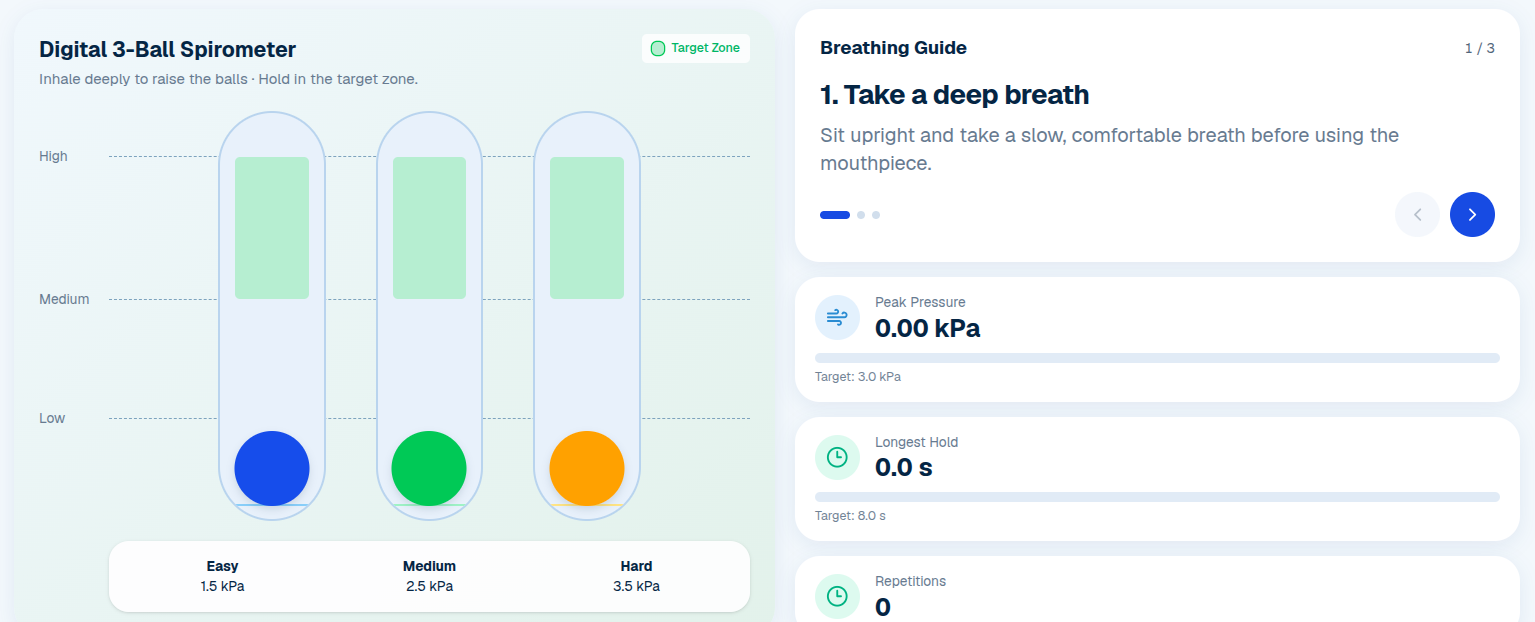
\includegraphics[height=3.3cm]{figures/session.png}\hfill
  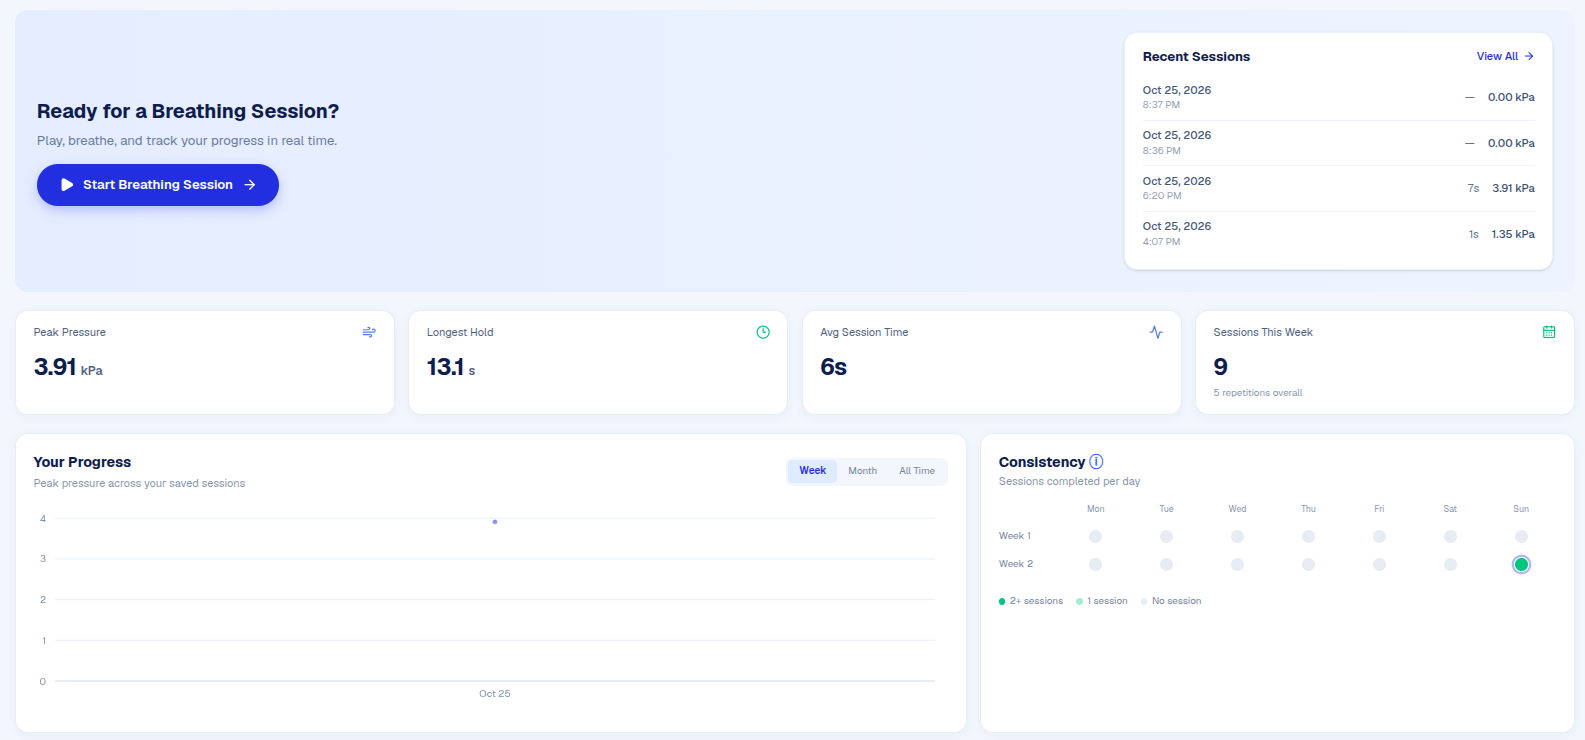
\includegraphics[height=3.3cm]{figures/dashboard.png}
  \caption{The web application. Left: the breathing session screen with three virtual balls and live metrics. Right: the personal dashboard with summary cards, progress chart and consistency tracker.}
  \label{fig:screens}
\end{figure}

\subsection{Next Steps}

\begin{itemize}
  \item Send progress reports directly to the doctor, and add a doctor view for remote monitoring.
  \item Run a hospital pilot with patients. This needs a partner hospital and ethics approval.
  \item Replace the pressure sensor with a high-accuracy airflow sensor, subject to funding.
  \item Build a standalone device with a built-in speaker and battery, so that no laptop is needed.
\end{itemize}

\subsection{Sensor Selection: What We Tried}
\label{sec:sensors}

Our device needs to measure how strongly the user breathes, so that the virtual balls rise and fall with the breath. We needed a sensor that measures either the airflow or the change in air pressure inside the pipe. It also had to be small, work with a microcontroller and fit a student budget.

We searched datasheets from Honeywell and Sensirion, online stores (Robu, Mouser, DigiKey, Element14 and Amazon), electronics shops in Hyderabad and the ECE store catalogue. We also discussed the options with faculty members and ECE lab staff. We tried four approaches before reaching our final design.

\textbf{Approach 1: Commercial airflow and pressure sensors (not used).} We first studied the sensors used in medical ventilators and spirometers, such as the Honeywell Zephyr and AWM5000 airflow sensors, the Honeywell ABP and HSC pressure sensors, and the Sensirion SFM3000 and SDP810 sensors. These sensors are accurate, but they were too costly for us. The ECE coordinator approved a budget of more than \rupee 3,000 for the project. Even so, the models priced around \rupee 3,000 were out of stock in every store we checked, and the models in stock cost more than \rupee 7,000.

\textbf{Approach 2: Venturi tube with two pressure sensors (not used).} A Venturi tube has a narrow section in the middle. Air speeds up in the narrow part and its pressure drops, so the pressure difference between the wide and narrow parts gives the airflow. We calculated the expected pressure difference for our setup. Because breathing through an incentive spirometer is gentle, the difference was too small for low-cost sensors to measure reliably, and the balls could not move smoothly. Published work reports the same problem: measurement error grows sharply at low flows \cite{edmunds}.

\textbf{Approach 3: Turbine airflow sensors (not used).} We tested water-flow and airflow sensors from the SCRC lab. They contain a small fan that spins when air passes through. The fan needs a strong flow to start turning, and its readings were inaccurate at low flow. Our users are patients with weak breathing, so these sensors were not suitable.

\textbf{Approach 4: One pressure sensor in a closed pipe (chosen).} When the far end of the pipe is closed, the air inside forms a closed system, and each breath changes the pressure throughout the whole pipe. One sensor at any point is then enough. We first considered an electronic valve to close the far end, but no suitable valve was available in time, so we use the spirometer body itself as the air container. We made a small hole in the pipe, fitted the HX710B air pressure sensor from the ECE store (a 24-bit module of about 19.6~mm $\times$ 13.5~mm), sealed it, and calibrated its readings. This design is low in cost, uses a part that was available immediately, and works at the low effort levels that patients produce.

\subsection{Testing}
\label{sec:testing}

\textbf{Calibration.} We calibrated the sensor against a real 3-ball spirometer. We breathed through the device, watched how high the balls rose, and recorded the sensor reading at each ball level. We repeated this over several trials to check that the readings were consistent. The balls respond to airflow while the sensor measures pressure, so the two were compared carefully when setting the prototype thresholds.

\textbf{End-to-end testing.} We tested the full chain: sensor, Arduino, bridge, web application, music and dashboard. Before saving, the server checks every session and rejects invalid data, such as a pressure outside 0--5~kPa or a repetition time outside the session.

\subsection{Research basis}
\label{sec:research}

\begin{itemize}
  \item \textbf{Music biofeedback} \cite{bhandari}: in a study of 28 people, breath-linked feedback slowed breathing to about 6--7 breaths per minute and raised heart-rate variability by about 30\%. Music alone had no effect, and all 7 users in the music-feedback group said they would use the application.
  \item \textbf{Electronic incentive spirometer} \cite{silva}: a sensor added to a 3-ball spirometer showed that heavier balls need more pressure, not proportionally more flow. This supports our pressure-based levels and calibration on the real device.
  \item \textbf{Low-cost pressure spirometry} \cite{edmunds}: a tube, pressure sensor and Arduino for under \$50. Simple threshold-based breath detection matched detailed analysis within 2\%, which supports our repetition counting.
  \item \textbf{Frugal Arduino spirometer} \cite{wallace}: a \pounds 45 device agreed closely with a certified spirometer (ICC 0.97), showing that frugal designs can be clinically meaningful.
  \item \textbf{Music in medical devices}: Lenire \cite{lenire}, MedRhythms \cite{medrhythms}, the Pacifier Activated Lullaby \cite{pal}, Sensate \cite{sensate} and raga therapy \cite{raga}.
\end{itemize}

\textbf{Limitation and planned sensor upgrade.} An airflow sensor is the preferred sensor for this device, because it measures the flow of each breath directly, and the volume of air inhaled can be calculated from it. For the prototype, we used a pressure sensor and calibrated it against a real 3-ball spirometer, because suitable airflow sensors were not available within our budget (Section~\ref{sec:sensors}). Breathing pressure reflects the patient's effort, so the current prototype is a therapy and tracking aid and not a diagnostic spirometer.

With adequate funding, we will replace the pressure sensor with a high-accuracy, medical-grade airflow sensor, such as the Honeywell Zephyr or Sensirion SFM3000 series. Each of these sensors costs about \rupee 7,000. This upgrade will make the readings more accurate and clinically meaningful. Clinical targets will be set with doctors during the pilot study.

% =====================================================================
\section{Beneficiaries and Impact}

\begin{itemize}
  \item \textbf{Patients.} The 3-part harmony rewards every good breath. Because the exercise is no longer boring, patients do more repetitions, hold each breath longer, and inhale and exhale more air. Regular practice helps the lungs expand and can lower the risk of lung problems after surgery.
  \item \textbf{Doctors, nurses and physiotherapists.} They can follow each patient's daily progress through recorded metrics: how often, how strongly and how long the patient breathes. Patients can share downloaded progress reports with them today. With the planned direct-sharing feature, reports will reach the doctor automatically, so they can monitor patients remotely and act early when a patient skips exercises or stops improving.
  \item \textbf{Hospitals and the health system.} Better adherence can mean fewer complications and shorter hospital stays. BreathNote reuses the spirometer that hospitals already buy, so the upgrade cost is small.
  \item \textbf{Families and caregivers.} They can check that the exercise is being done at home.
  \item \textbf{Learning.} The music itself teaches the correct technique: slow, deep and sustained breathing.
\end{itemize}

% =====================================================================
\section{Estimated Cost}

\begin{table}[h]
\centering
\caption{Approximate cost of one prototype unit (Indian market prices).}
\label{tab:cost}
\small
\begin{tabularx}{0.75\linewidth}{@{}L r@{}}
\toprule
\textbf{Item} & \textbf{Cost (Rs.)} \\
\midrule
3-ball incentive spirometer                    & 300--400 \\
HX710B pressure sensor module                  & 150--250 \\
Arduino Uno (compatible board)                 & 500--800 \\
Tube, mouthpiece, wires, breadboard, USB cable & 200--300 \\
\midrule
\textbf{Total per prototype unit}              & \textbf{1,150--1,750} \\
\bottomrule
\end{tabularx}
\end{table}

\begin{itemize}
  \item \textbf{Software:} built with free, open-source tools. The database runs on a free cloud plan during testing, so the running cost is nearly \rupee 0 at present.
  \item \textbf{Future standalone device:} an ESP32 board with Bluetooth and Wi-Fi, a speaker, a battery and a casing. Estimated \rupee 2,000--2,500 per unit in small batches, and lower in bulk. A high-accuracy airflow sensor would add about \rupee 7,000 per unit.
  \item \textbf{Running cost at scale:} about \rupee 1,000--3,000 per month for cloud hosting for the first few thousand users (our assumption).
\end{itemize}

% =====================================================================
\Needspace{16\baselineskip}
\section{Implementation and Scale-up Plan}

\begin{table}[H]
\centering
\caption{Rollout plan.}
\label{tab:roadmap}
\small
\begin{tabularx}{\linewidth}{@{}P{3.6cm} P{2.4cm} L@{}}
\toprule
\textbf{Phase} & \textbf{Timeline} & \textbf{Main activities} \\
\midrule
1. Deployment and doctor monitoring & About 3 months & Deploy the web application on a secure cloud server; send progress reports directly to the doctor; doctor view to monitor patients remotely \\
2. Hospital pilot           & 3--6 months     & Partner hospital and ethics approval; testing with post-surgery patients; comparison of results with and without music \\
3. Standalone device        & After the pilot & Wi-Fi module (ESP32) in place of the Arduino; 3D-printed air chamber with an electronic valve; airflow sensor; built-in speaker and battery; mobile application \\
4. Scale-up                 & Growth stage    & Multi-hospital doctor portal with weekly reports; clip-on add-on with spirometer manufacturers; hospitals, home-care providers and tele-rehabilitation programmes \\
\bottomrule
\end{tabularx}
\end{table}

\Needspace{8\baselineskip}
\textbf{Why the solution can scale.}
\begin{itemize}
  \item It reuses a low-cost device that hospitals already stock, so staff need no new training.
  \item The software is web-based and, once deployed, will run in the cloud. One system can serve many hospitals, and each user's data stays private.
  \item Targets and the base note are set in one file, so each patient or hospital can adjust them.
  \item The music can be extended to more musical styles, and the application to Indian languages.
  \item The low unit cost suits district hospitals, rural health centres and homes.
\end{itemize}

% =====================================================================
\Needspace{10\baselineskip}
\section{Planned Enhancements}

The current prototype proves the concept. The following enhancements will turn BreathNote into a complete, standalone device. They will be carried out in Phases 1 and 3 of the rollout plan (Table~\ref{tab:roadmap}).

\begin{enumerate}
  \item \textbf{Wireless data transfer.} The Arduino and the USB cable will be removed. A Wi-Fi module, such as an ESP32 board, will read the sensor and send the data directly to the web application over Wi-Fi. The device will no longer need to be connected to a laptop.
  \item \textbf{Deployment of the web application.} At present, the web application runs locally on a laptop during testing. It will be deployed on a secure cloud hosting service with a public web address (HTTPS), so that patients and doctors can use it from any phone, tablet or computer. Together with the Wi-Fi module, this will allow the device to send each session to the online application from any location.
  \item \textbf{Remote monitoring by the doctor.} A doctor view will be added to the web application. Progress reports will be sent directly to the doctor, who will be able to see each patient's daily metrics, consistency and history remotely, without an in-person visit.
  \item \textbf{Custom air chamber with an electronic valve.} At present, the body of the 3-ball spirometer serves as the air container that closes the far end of the pipe. We will design our own air chamber, produce it by 3D printing, and close the far end of the pipe with an electronically controlled valve. BreathNote will then be a complete electronic device that does not depend on a conventional spirometer.
  \item \textbf{Airflow sensor in place of the pressure sensor.} The pressure sensor will be replaced with a high-accuracy, medical-grade airflow sensor, which costs about \rupee 7,000 per unit. It will measure the flow of each breath directly, and the volume of air inhaled can be calculated from it. This upgrade depends on funding (Section~\ref{sec:research}).
\end{enumerate}

% =====================================================================
\section{Potential Adopters}

\begin{itemize}
  \item \textbf{Hospitals:} surgery, cardiothoracic, pulmonology and ICU departments in government and private hospitals.
  \item \textbf{Physiotherapy and pulmonary rehabilitation centres}, and home-care providers after discharge.
  \item \textbf{Medical device companies} that already make incentive spirometers, to offer BreathNote as a smart clip-on add-on.
  \item \textbf{Government health programmes:} Ayushman Arogya Mandirs for low-cost rehabilitation in rural areas; the Ayushman Bharat Digital Mission to link progress reports with digital health records; and eSanjeevani for remote monitoring by doctors.
  \item \textbf{Medical colleges and research institutes}, for clinical studies on adherence and music therapy.
  \item \textbf{Music therapy groups and music institutions}, to build a library of therapy music.
\end{itemize}

% =====================================================================
\begin{thebibliography}{99}
\footnotesize
\setlength{\itemsep}{0pt}

\bibitem{cleveland} Cleveland Clinic. \textit{Incentive Spirometer.} \url{https://my.clevelandclinic.org/health/drugs/4302-incentive-spirometer}

\bibitem{silva} L.~Silva, R.~Shur, W.~Ganley and J.~Shur. \textit{Measuring Breath Profiles Using an Electronic Incentive Spirometer.} Conference poster, 2024.

\bibitem{edmunds} J.~L.~Edmunds et al. \textit{Low-Cost Differential Pressure Spirometry for Emergency Ventilator Tidal Volume Sensing.} medRxiv preprint, 2020. doi:10.1101/2020.09.25.20198069.

\bibitem{wallace} J.~Wallace et al. \textit{A Frugal Arduino-Based Spirometer for Low-Resource Settings: Design, Development and Validation of a Preliminary Prototype.} Frontiers in Bioengineering and Biotechnology 13:1664127, 2026. doi:10.3389/fbioe.2025.1664127.

\bibitem{bhandari} R.~Bhandari, A.~Parnandi, E.~Shipp, B.~Ahmed and R.~Gutierrez-Osuna. \textit{Music-Based Respiratory Biofeedback in Visually-Demanding Tasks.} Proceedings of New Interfaces for Musical Expression (NIME), 2015.

\bibitem{lenire} Lenire: tinnitus treatment using bimodal neuromodulation. \url{https://www.lenire.com/}

\bibitem{medrhythms} MedRhythms: digital neurorehabilitation platform. \url{https://medrhythms.com/}

\bibitem{pal} NeoLight: Pacifier Activated Lullaby (P.A.L.). \url{https://theneolight.com/product-pages/p-a-l}

\bibitem{sensate} Sensate: vagus nerve toning device. \url{https://www.getsensate.com/}

\bibitem{raga} \textit{Raga Therapy: A Complementary Approach to Disease Management Through Indian Classical Music.} ResearchGate.

\end{thebibliography}

\end{document}
